\documentclass[crop, tikz]{standalone}
\usepackage{tikz}

\begin{document}
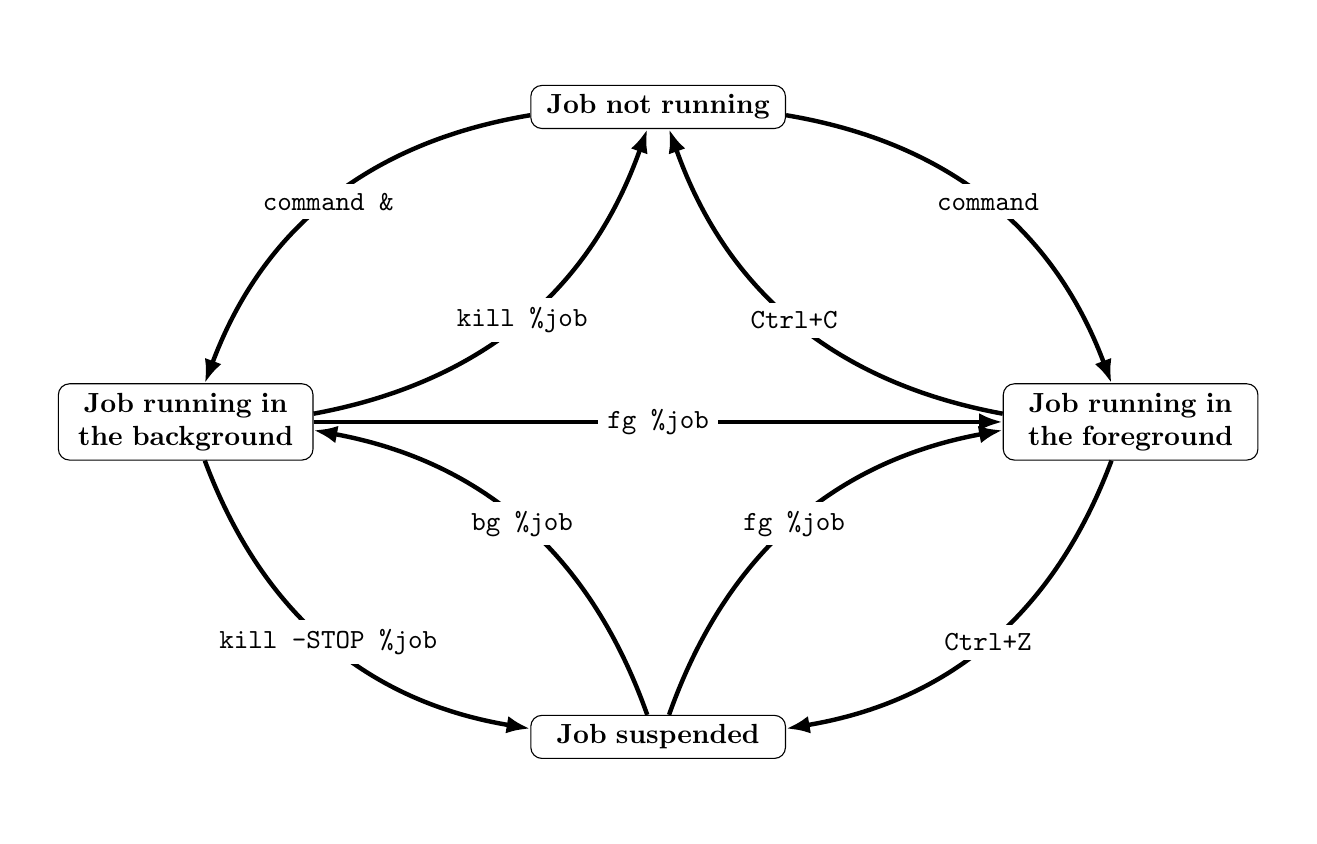
\begin{tikzpicture}
\usetikzlibrary{arrows.meta}

% Just a workaround to leave some space around the diagram
\filldraw[color=white,fill=white] (-8,-9) rectangle (8,1);

% Boxes
\newcommand{\tbox}[3]{
	\node[draw, rounded corners, text centered, text width=3cm]
		(#1) at (#2) {\bf #3}
	;
}
\tbox  {top}    {0,0}     {Job not running}
\tbox  {left}   {-6,-4}   {Job running in the background}
\tbox  {right}  {6,-4}    {Job running in the foreground}
\tbox  {bottom} {0,-8}    {Job suspended}

% Arrows
\newcommand{\arr}[4]{
	\draw[-{Latex[length=3mm]}, ultra thick]
		(#1) edge[#4] node[fill=white] {\texttt{#3}} (#2)
	;
}
\arr  {top}    {left}   {command \&}       {bend right}
\arr  {left}   {top}    {kill \%job}       {bend right}
\arr  {left}   {bottom} {kill -STOP \%job} {bend right}
\arr  {bottom} {left}   {bg \%job}         {bend right}
\arr  {bottom} {right}  {fg \%job}         {bend left}
\arr  {right}  {bottom} {Ctrl+Z}           {bend left}
\arr  {right}  {top}    {Ctrl+C}           {bend left}
\arr  {top}    {right}  {command}          {bend left}
\arr  {left}   {right}  {fg \%job}         {}
\end{tikzpicture}
\end{document}
